%!TEX spellcheck
%%%%%%%%%%%%%%%%%%%%%%%%%%%%%%%%%%%%%%%%%
% Beamer Presentation
% LaTeX Template
% Version 2.0 (March 8, 2022)
%
% This template originates from:
% https://www.LaTeXTemplates.com
%
% Author:
% Vel (vel@latextemplates.com)
%
% License:
% CC BY-NC-SA 4.0 (https://creativecommons.org/licenses/by-nc-sa/4.0/)
%
%%%%%%%%%%%%%%%%%%%%%%%%%%%%%%%%%%%%%%%%%

%----------------------------------------------------------------------------------------
%	PACKAGES AND OTHER DOCUMENT CONFIGURATIONS
%----------------------------------------------------------------------------------------

\documentclass[
	11pt, % Set the default font size, options include: 8pt, 9pt, 10pt, 11pt, 12pt, 14pt, 17pt, 20pt
	%t, % Uncomment to vertically align all slide content to the top of the slide, rather than the default centered
	%aspectratio=169, % Uncomment to set the aspect ratio to a 16:9 ratio which matches the aspect ratio of 1080p and 4K screens and projectors
	handout,
]{beamer}

\graphicspath{{Images/}{./}} % Specifies where to look for included images (trailing slash required)

\usepackage{booktabs} % Allows the use of \toprule, \midrule and \bottomrule for better rules in tables

%----------------------------------------------------------------------------------------
%	SELECT LAYOUT THEME
%----------------------------------------------------------------------------------------

% Beamer comes with a number of default layout themes which change the colors and layouts of slides. Below is a list of all themes available, uncomment each in turn to see what they look like.

%\usetheme{default}
%\usetheme{AnnArbor}
%\usetheme{Antibes}
%\usetheme{Bergen}
%\usetheme{Berkeley}
%\usetheme{Berlin}
%\usetheme{Boadilla}
%\usetheme{CambridgeUS}
%\usetheme{Copenhagen}
%\usetheme{Darmstadt}
%\usetheme{Dresden}
%\usetheme{Frankfurt}
%\usetheme{Goettingen}
%\usetheme{Hannover}
%\usetheme{Ilmenau}
%\usetheme{JuanLesPins}
%\usetheme{Luebeck}
\usetheme{Madrid}
%\usetheme{Malmoe}
%\usetheme{Marburg}
%\usetheme{Montpellier}
%\usetheme{PaloAlto}
%\usetheme{Pittsburgh}
%\usetheme{Rochester}
%\usetheme{Singapore}
%\usetheme{Szeged}
%\usetheme{Warsaw}

%----------------------------------------------------------------------------------------
%	SELECT COLOR THEME
%----------------------------------------------------------------------------------------

% Beamer comes with a number of color themes that can be applied to any layout theme to change its colors. Uncomment each of these in turn to see how they change the colors of your selected layout theme.

%\usecolortheme{albatross}
%\usecolortheme{beaver}
%\usecolortheme{beetle}
%\usecolortheme{crane}
%\usecolortheme{dolphin}
%\usecolortheme{dove}
%\usecolortheme{fly}
%\usecolortheme{lily}
%\usecolortheme{monarca}
%\usecolortheme{seagull}
%\usecolortheme{seahorse}
%\usecolortheme{spruce}
%\usecolortheme{whale}
%\usecolortheme{wolverine}

%----------------------------------------------------------------------------------------
%	SELECT FONT THEME & FONTS
%----------------------------------------------------------------------------------------

% Beamer comes with several font themes to easily change the fonts used in various parts of the presentation. Review the comments beside each one to decide if you would like to use it. Note that additional options can be specified for several of these font themes, consult the beamer documentation for more information.

\usefonttheme{default} % Typeset using the default sans serif font
%\usefonttheme{serif} % Typeset using the default serif font (make sure a sans font isn't being set as the default font if you use this option!)
%\usefonttheme{structurebold} % Typeset important structure text (titles, headlines, footlines, sidebar, etc) in bold
%\usefonttheme{structureitalicserif} % Typeset important structure text (titles, headlines, footlines, sidebar, etc) in italic serif
%\usefonttheme{structuresmallcapsserif} % Typeset important structure text (titles, headlines, footlines, sidebar, etc) in small caps serif

%------------------------------------------------

%\usepackage{mathptmx} % Use the Times font for serif text
\usepackage{palatino} % Use the Palatino font for serif text
\usepackage{hyperref}
%\usepackage{helvet} % Use the Helvetica font for sans serif text
\usepackage[default]{opensans} % Use the Open Sans font for sans serif text
%\usepackage[default]{FiraSans} % Use the Fira Sans font for sans serif text
%\usepackage[default]{lato} % Use the Lato font for sans serif text
\usepackage{ctex}
\usepackage{siunitx}
\usepackage{tabularx}
\usepackage{umoline}
\usepackage{fourier}
%----------------------------------------------------------------------------------------
%	SELECT INNER THEME
%----------------------------------------------------------------------------------------

% Inner themes change the styling of internal slide elements, for example: bullet points, blocks, bibliography entries, title pages, theorems, etc. Uncomment each theme in turn to see what changes it makes to your presentation.

%\useinnertheme{default}
\useinnertheme{circles}
%\useinnertheme{rectangles}
%\useinnertheme{rounded}
%\useinnertheme{inmargin}

%----------------------------------------------------------------------------------------
%	SELECT OUTER THEME
%----------------------------------------------------------------------------------------

% Outer themes change the overall layout of slides, such as: header and footer lines, sidebars and slide titles. Uncomment each theme in turn to see what changes it makes to your presentation.

%\useoutertheme{default}
%\useoutertheme{infolines}
%\useoutertheme{miniframes}
%\useoutertheme{smoothbars}
%\useoutertheme{sidebar}
%\useoutertheme{split}
%\useoutertheme{shadow}
%\useoutertheme{tree}
%\useoutertheme{smoothtree}

%\setbeamertemplate{footline} % Uncomment this line to remove the footer line in all slides
%\setbeamertemplate{footline}[page number] % Uncomment this line to replace the footer line in all slides with a simple slide count

%\setbeamertemplate{navigation symbols}{} % Uncomment this line to remove the navigation symbols from the bottom of all slides

%----------------------------------------------------------------------------------------
%	PRESENTATION INFORMATION
%----------------------------------------------------------------------------------------

\title[Data Analysis]{Data Analysis} % The short title in the optional parameter appears at the bottom of every slide, the full title in the main parameter is only on the title page

\subtitle{数据分析} % Presentation subtitle, remove this command if a subtitle isn't required

\author[张凡]{张凡} % Presenter name(s), the optional parameter can contain a shortened version to appear on the bottom of every slide, while the main parameter will appear on the title slide

\institute[XDF]{新东方国际教育 \\ \smallskip \textit{zhangfan@xdf.cn}} % Your institution, the optional parameter can be used for the institution shorthand and will appear on the bottom of every slide after author names, while the required parameter is used on the title slide and can include your email address or additional information on separate lines

\date[\today]{GRE 冲分班数学 \\ \today} % Presentation date or conference/meeting name, the optional parameter can contain a shortened version to appear on the bottom of every slide, while the required parameter value is output to the title slide

%----------------------------------------------------------------------------------------


%----------------------------------------------------------------------------------------
%	Section Slide
%----------------------------------------------------------------------------------------
\AtBeginSection[]{
  \begin{frame}
  \vfill
  \centering
  \begin{beamercolorbox}[sep=8pt,center,shadow=true,rounded=true]{title}
    \usebeamerfont{title}\insertsectionhead\par%
  \end{beamercolorbox}
  \vfill
  \end{frame}

%----------------------------------------------------------------------------------------
%	TABLE OF CONTENTS SLIDE OF THE CURRENT SECTION
%----------------------------------------------------------------------------------------
	\begin{frame}
		\frametitle{Presentation Overview for \secname} % Slide title, remove this command for no title
		\tableofcontents[currentsection, hideothersubsections, sectionstyle=show/show]
	\end{frame}
  }

%----------------------------------------------------------------------------------------

\AtBeginSubsection[]{
  \begin{frame}
  \vfill
  \centering
    \usebeamerfont{title}\insertsubsectionhead\par%
  \vfill
  \end{frame}
}
%----------------------------------------------------------------------------------------


\begin{document}

%----------------------------------------------------------------------------------------
%	TITLE SLIDE
%----------------------------------------------------------------------------------------

\begin{frame}
	\titlepage % Output the title slide, automatically created using the text entered in the PRESENTATION INFORMATION block above
\end{frame}



%----------------------------------------------------------------------------------------
%	PRESENTATION BODY SLIDES
%---------------------------------------------------------------------------------------

\section{Counting Methods}

%------------------------------------------------

\subsection{Lists}
\begin{frame}
	\frametitle{Lists} % Slide title, remove this command for no title
	\framesubtitle{列表:有顺序可重复}
	\begin{definition}
		\begin{itemize}
			\item In a list, the members are ordered—that is, rearranging the members of a list makes it a different list.
			\item Elements can be repeated in a list and the repetitions matter.
		\end{itemize}
	\end{definition}
	\begin{example}
		1, 2, 3 and 2, 3, 1 and 1, 1, 2, 3 are all different list. 
	\end{example}
\end{frame}

%------------------------------------------------

\subsection{Sets}
\begin{frame}
	\frametitle{Sets} % Slide title, remove this command for no title
	\framesubtitle{集合:无顺序不可重复}
	\begin{definition}
		\begin{itemize}
			\item In a set, repetitions are
not counted as additional elements.
			\item the order of the elements does not
matter.
		\end{itemize}
	\end{definition}
	\begin{example}
		{1, 2, 3} and {2, 3, 1} and {1, 1, 2, 3} are the same set. 
	\end{example}
\end{frame}

%------------------------------------------------

\begin{frame}
	\frametitle{Subsets} % Slide title, remove this command for no title
	\framesubtitle{空集是任意集合的子集}
	\begin{definition}
	If A and B are sets and all of the
members of A are also members of B, then A is a subset of B. By convention, $\emptyset$ is a subset of
every set.
	\end{definition}
	\begin{example}
		{2, 8} is a subset of {0, 2, 4, 6, 8}.
	\end{example}

	\begin{theorem}
		If a set has n elements, then the number of subset of the given set is $2^n$
	\end{theorem}
	\alert{We will prove the above theorem by induction when we talk about Combinations.}
\end{frame}

%------------------------------------------------


\begin{frame}
	\frametitle{The Operations of Sets} % Slide title, remove this command for no title
	\framesubtitle{交集并集}
	\begin{definition}
If S and T are sets, then the
intersection of S and T is the set of all elements that are in both S and T and
is denoted by $S\cap	T$
	\end{definition}
	\begin{example}
		{2, 8} is a subset of {0, 2, 4, 6, 8}.
	\end{example}

	\begin{theorem}
		If a set has n elements, then the number of subset of the given set is $2^n$
	\end{theorem}
	\alert{We will prove the above theorem by induction when we talk about Combinations.}
\end{frame}

%------------------------------------------------

\subsection{Addition Principle}

%------------------------------------------------

\begin{frame}
	\frametitle{Addition Principle} % Slide title, remove this command for no title
	\framesubtitle{加法原则}
	\begin{definition}
		\begin{itemize}
			\item Suppose there are two choices to be made sequentially.
			\item Suppose also that there are $k$ different possibilities for the first choice and $m$ different possibilities for the second choice for each possibilities of the first choice. 
		\end{itemize}
				Then, \alert{under those conditions}, there are $k\cdot m$ different possibilities for the pair of choices.
	\end{definition}
	\begin{example}
	For a 6 digit Bank PIN, there could be $10^6$ different passwords. 
	\end{example}
\end{frame}

%------------------------------------------------

\subsection{Multiplication Principle}

%------------------------------------------------
% The relation between addition and multiplication

\begin{frame}
	\frametitle{Multiplication Principle} % Slide title, remove this command for no title
	\framesubtitle{乘法原则}
	\begin{definition}
		\begin{itemize}
			\item Suppose there are two choices to be made sequentially.
			\item Suppose also that there are $k$ different possibilities for the first choice and $m$ different possibilities for the second choice for each possibilities of the first choice. 
		\end{itemize}
				Then, \alert{under those conditions}, there are $km$ different possibilities for the pair of choices.
	\end{definition}
	\begin{example}
	For a 6 digit Bank PIN, there could be $10^6$ different passwords. 
	\end{example}
\end{frame}

%------------------------------------------------

\begin{frame}
	\frametitle{The Decision Tree} % Slide title, remove this command for no title
	\framesubtitle{决策树}
	What if a 6 digit Bank PIN can not start or end with 0?

	\bigskip \bigskip
	\pause Can you draw the decision tree?
\end{frame}

%------------------------------------------------

%TODO: the independen condition

\begin{frame}
	\frametitle{Have a try!}
	\framesubtitle{}
A man walks to his home from his current location on the rectangular grid shown. If
he may choose to walk north or east at any corner, but may never moves south or
west. How many different paths can the man take to get home?
	\begin{figure}
		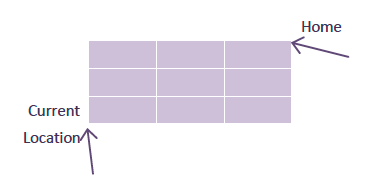
\includegraphics[width=0.5\linewidth]{Man_Walk.png}
	\end{figure}
\bigskip
\pause
Answer \textbf{$2^3$}
\bigskip

\end{frame}

%------------------------------------------------

\begin{frame}
	\frametitle{Demo}
	\framesubtitle{难题演示}
\textbf{GMAT-OG} In a meeting of 3 representatives from each of 6 different companies, each person
shook hands with every person not from his or her own company. If the representatives did not shake hands with people from their own company, how many handshakes took place?
	\begin{columns}[t] 
		\begin{column}{0.5\textwidth} % Left column width
			\begin{enumerate}[A]
				\item 45
			  \item 135
			  \item 144
			  \item 270
			  \item 288
			\end{enumerate}
		\end{column}
		\begin{column}{0.5\textwidth} % Right column width
			\begin{figure}
				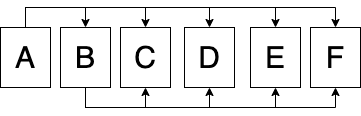
\includegraphics[width=0.5\linewidth]{Handshakes.png}
				\caption{Handshakes for Company A should be $3\times15 = 45$;Handshakes for Company B should be $3\times12 = 36$.}
			\end{figure}		
			$3 \times 15 + 3 \times 12 + 3\times 9 + 3 \times 6 + 3\times3 = 135$
			\pause
      Answer \textbf{B} 135 \pause 
		\end{column}
	\end{columns}
\end{frame}

%------------------------------------------------




\subsection{Permutations}

%------------------------------------------------

\begin{frame}
	\frametitle{A Vanilla Question} % Slide title, remove this command for no title
	\framesubtitle{排排坐的排法}
	\begin{columns}[t] 
		\begin{column}{0.3\textwidth} % Left column width
			How many kinds of different lists can be constructed 3 Students --- student A, student B and student C.  
		\end{column}
		\begin{column}{0.7\textwidth} % Right column width
		  \pause
			\begin{figure}
				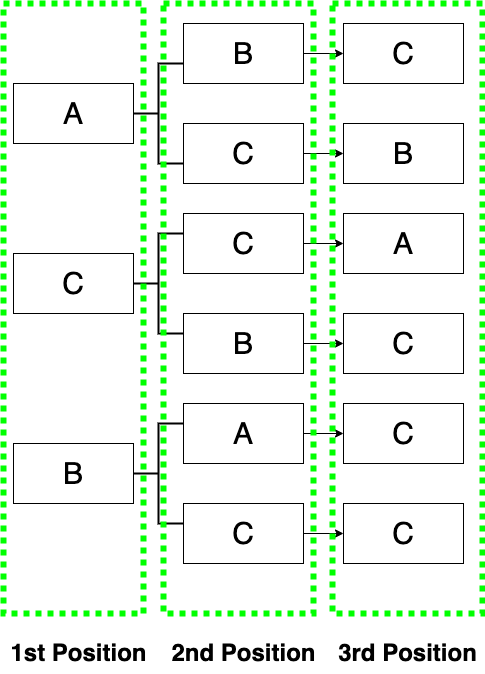
\includegraphics[width=0.5\linewidth]{Permutation3.png}
				\caption{6 Different Lists can be formed from 3 different students}
			\end{figure}
		\end{column}
	\end{columns}
\end{frame}


%------------------------------------------------

\begin{frame}
	\frametitle{A Vanilla Question} % Slide title, remove this command for no title
	\framesubtitle{排排坐的排法}
	\begin{columns}[t] 
		\begin{column}{0.3\textwidth} % Left column width
		   What about the 4 different students?\\
		   5 different students\\
		   6 different students\\
		   $\vdots$

		\end{column}
		\begin{column}{0.7\textwidth} % Right column width
		  \pause
		  \begin{equation*}
		  		  	4 \times 3 \times 2 \times 1 = 24 
		  \end{equation*}
		\end{column}
	\end{columns}
\end{frame}

%------------------------------------------------

\begin{frame}
	\frametitle{Permutation} % Slide title, remove this command for no title
	\framesubtitle{全排}
	\begin{definition}
		Suppose n objects are to be ordered from 1st to nth, then
 the number of ways the objects can be ordered is $n(n-1)(n-2)(n-3)\ldots1=n!$ 
	\end{definition}
\end{frame}

%------------------------------------------------

\begin{frame}
\frametitle{Have a try!}
\framesubtitle{把Bus Seats 编号}
\textbf{og-p463-1.7.16} Suppose that 10 students are going on a bus trip, and each
of the students will be assigned to one of the 10 available seats. What is  the
number of possible different seating arrangements of the students on the
bus?


\bigskip
\pause
$10! = 10 \times 9 \times 8 \times 7 \ldots 1 = 3,628,800  $\\
\bigskip\pause
Answer \textbf{3,628,800} \pause 
\end{frame}

%------------------------------------------------

\begin{frame}
	\frametitle{Have a try!}
	\framesubtitle{}
A gardener wishes to plant 5 bushes in straight row. Each bush has flowers of a
different solid color (white, yellow, pink, red, and purple). How many ways can the
bushes be arranged so that middle bush is the one with red flowers?
	\begin{figure}
		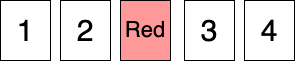
\includegraphics[width=0.3\linewidth]{Bushes.png}
		\caption{There are 4 vacancy.}
	\end{figure}
\begin{equation*}
	^5P_4 =\frac{5!}{(5-4)!} = 5! = 120
\end{equation*}
\bigskip
\pause
Answer \textbf{$120$}
\bigskip

\end{frame}

%------------------------------------------------

\begin{frame}
	\frametitle{A Real QR Problem!}
	\framesubtitle{}
	\begin{figure}
		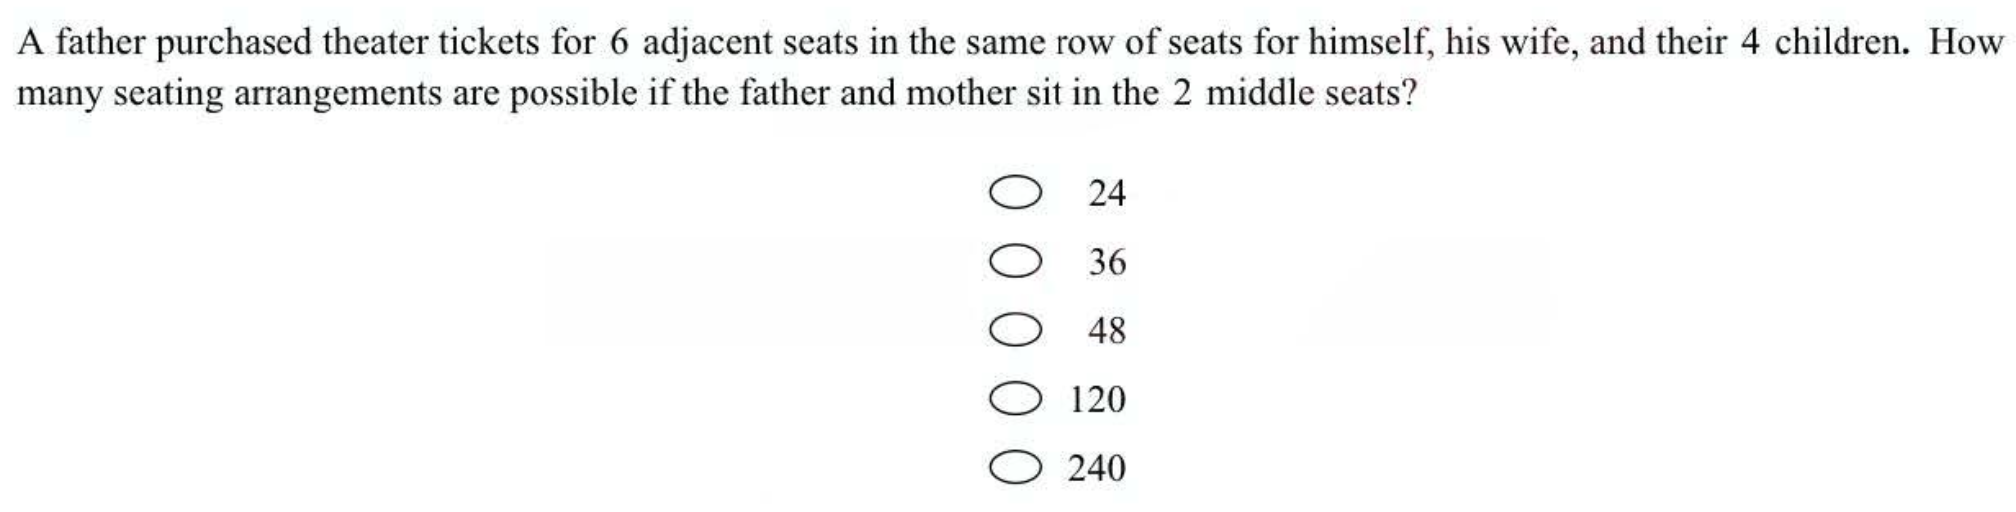
\includegraphics[width=\linewidth]{K-Permutation_Example_Question.png}
		\caption{8-Sec3-8}
	\end{figure}
	\pause
$Children's\ Permutation= 4! =24$\\
$Parents'\ Permutation= 2! =2$\\
$Possible Arrangements= (Children's\ Permutation) \cdot (Parents'\ Permutation) =4! \cdot 2!=48$\\

\pause
\bigskip
Answer \textbf{C}  48
\end{frame}


%------------------------------------------------

\subsection{K-Permutation}

%------------------------------------------------
 
 \begin{frame}
	\frametitle{A Vanilla Question} % Slide title, remove this command for no title
	\framesubtitle{选部分人排排坐的排法}
	 Suppose that there are 8 students and 5 students are selected going on a bus trip, and each
of the students will be assigned to one of the 5 available seats. What is  the
number of possible different seating arrangements of the students on the
bus?

	\begin{figure}
		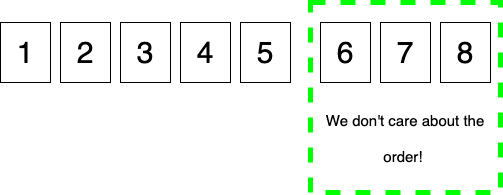
\includegraphics[width=0.5\linewidth]{K_permutation.png}
		\caption{The order about the final 3 students is irrelevant.}
	\end{figure}
	\begin{equation}
		\frac{8!}{3!} = \frac{8\times7\times6\cdots\times1}{3\times2\times1} = 6,720
	\end{equation}
\end{frame}

%------------------------------------------------

\begin{frame}
	\frametitle{K-Permutation} % Slide title, remove this command for no title
	\framesubtitle{K-全排}
	\begin{definition}
		Suppose that k objects will be selected from a set of n
objects, where , and the k objects will be placed in order from 1st to
kth, the number of ways to select and order k objects from a set of n objects is \\
\begin{equation*}
	^nP_k =\frac{n!}{(n-k)!}
\end{equation*}
	\end{definition}
\end{frame}

%------------------------------------------------


\begin{frame}
	\frametitle{Demo: K-Permutation} % Slide title, remove this command for no title
	\framesubtitle{难题演示}
	How many distinguished way to arrange the word “ORDER” if there are at least
	two letters between two “R”s?

		\begin{columns}[t] 
			\begin{column}{0.5\textwidth} % Left column width
				\begin{figure}
					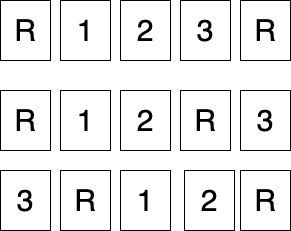
\includegraphics[width=0.8\linewidth]{ORDER.png}
					\caption{Three possible arrangements with blanks to fill}
				\end{figure}
			\end{column}
			\begin{column}{0.5\textwidth} % Right column width
				\begin{equation*}
					\begin{aligned}
						&^3P_3+ ^3P_2 \cdot 2 \\
						&=3! + \frac{3!}{2!} \cdot 2 \\
						&=18
					\end{aligned}
				\end{equation*}
			\end{column}
		\end{columns}
\end{frame}

%------------------------------------------------




\subsection{Combinations}

%------------------------------------------------
 
 \begin{frame}
	\frametitle{A Vanilla Question} % Slide title, remove this command for no title
	\framesubtitle{选部分人不讲顺序的排法}
	 Suppose that there are 8 students and 5 students are selected going on a bus trip. What is  the
number of possible combinations of the students on the for the bus trip?

	\begin{figure}
		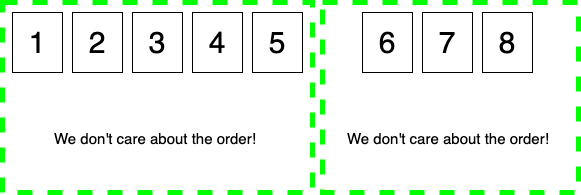
\includegraphics[width=0.5\linewidth]{Combination_8_5.png}
		\caption{The order about the  3 students abandoned and the 5 students chosen is irrelevant.}
	\end{figure}
	\begin{equation}
		\frac{8!}{5! 3!} = \frac{8\times7\times6\cdots\times1}{(5\times4\times3\times2\times1)(3\times2\times1)} = 56
	\end{equation}
\end{frame}

%------------------------------------------------

\begin{frame}
	\frametitle{Combinations} % Slide title, remove this command for no title
	\framesubtitle{n选k,不讲顺序}
	\begin{definition}
		Suppose that k objects will be chosen from a set of n
		objects, where , but that the k objects will not be put in order. The
		 the number of combinations of n objects taken k at a time and is \\
		\begin{equation*}
		  ^nC_k =\frac{n!}{k!(n-k)!}
		\end{equation*}
	\end{definition}

	\begin{proof}
		\begin{equation*}
			\begin{aligned}
				&(number\ of\ ways\ to\ select\ without\ order)\ \times\ (number\ of\ ways\ to\ order)\\ =
&(number\ of\ ways\ to\ select\ with\ order)\\
&(number\ of\ ways\ to\ select\ without\ order) =\\
&\frac{(number\ of\ ways\ to\ select\ with\ order)}{(number\ of\ ways\ to\ order)}
			\end{aligned}
		\end{equation*}
	\end{proof}
\end{frame}

%------------------------------------------------

\begin{frame}
	\frametitle{Have a try!}
	\framesubtitle{}
Suppose you want to select a 3-person committee from a
group of 9 students. How many ways are there to do this?
\pause
\begin{equation*}
	^9C_3 =\frac{9!}{3!6!} = 84
\end{equation*}
\bigskip
\pause
Answer \textbf{$84$} 
\end{frame}

%------------------------------------------------

\begin{frame}
	\frametitle{Rules of Combination}
	\framesubtitle{快速计算规则}
	\begin{itemize}
		\item $^nC_0=1$
		\item $^nC_1=n$ 
		\item $^nC_r = ^nC_{n-r}$ 
	\end{itemize}
\end{frame}

% TODO: Subset proof
\begin{frame}
	\frametitle{Have a try!}
	\framesubtitle{}
There are five points on line $l_1$ and four points on $l_2$. If $l_1$ and $l_2$ are parallel, how
many different triangles can be constructed based on these nine points?
  \pause
	\begin{figure}
		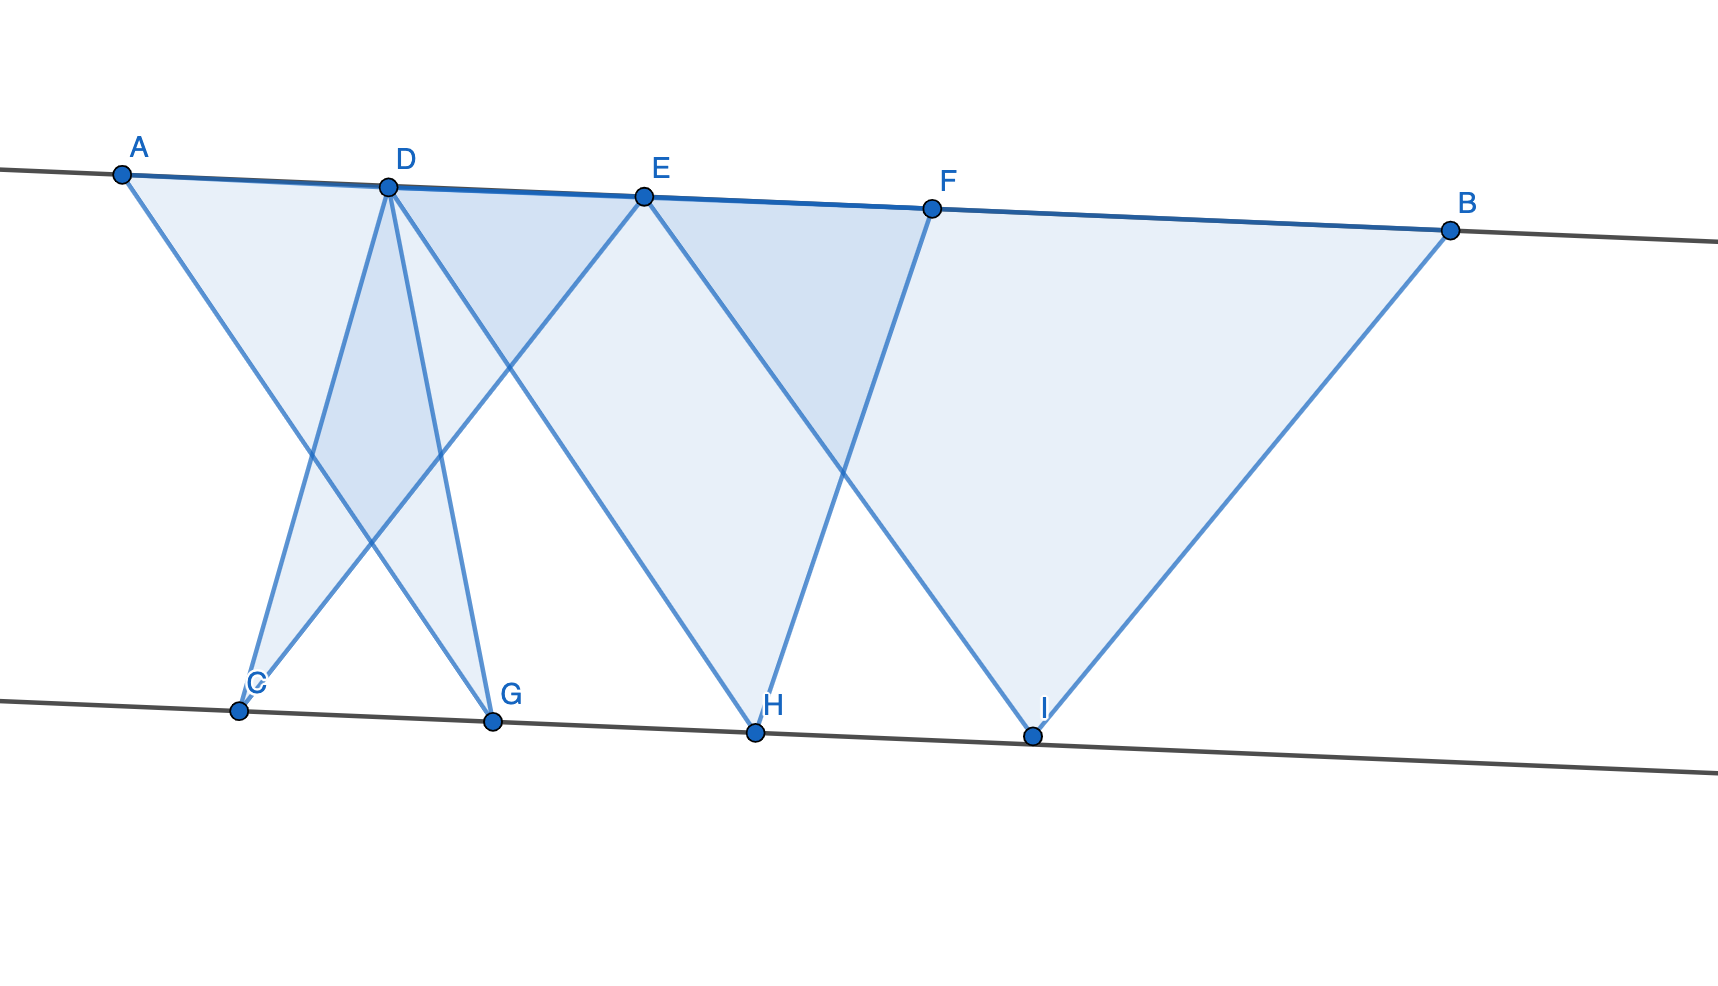
\includegraphics[width=0.5\linewidth]{Triangles_Combinations.png}
	\end{figure}

	$$^2C_5 \cdot ^1C_4 + ^1C_5 \cdot^2C_4 = 70$$  
	\bigskip
	\pause
Answer \textbf{$70$} 
\end{frame}

%------------------------------------------------


\begin{frame}
	\frametitle{Demo}
	\framesubtitle{反其道而行之:用总数去减}
\textbf{GMAT-鸡精} In a certain class of 20 students with different initials of surname, the roster is arranged by the order of initial of surnames. If three students are selected to join a
seminar, how many different ways to select them whose initial of surnames are not
near to each other?
	\begin{columns}[t] 
		\begin{column}{0.3\textwidth} % Left column width
				\begin{figure}
				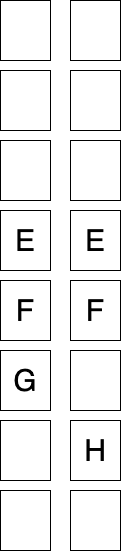
\includegraphics[width=0.2\linewidth]{Surnames.png}
				\caption{Two combinations that are not allowed.}
				\end{figure}		
		\end{column}
		\begin{column}{0.7\textwidth} % Right column width
		Case 1: Three consecutive initials\\
		$Combination_1 = 18$\\
		\bigskip
		Case 2: Only two consecutive initials \\
		Case 2-1: the two consecutive initials occupies the start or the end of the roster\\
		$Combination_{2-1} = 2 \times 17 = 34$\\
		Case 2-2: the two consecutive initials occupies neither the start nor the end of the roster\\
		$Combination_{2-2} = 17 \times 16 = 186$\\
		$\therefore ^3C_{20} - Combination_1 -Combination_{2-1} - Combination_{2-2} = 1140 - 18 - 34 - 186 = \textbf{902}$
		\end{column}
	\end{columns}
\end{frame}

%------------------------------------------------

\begin{frame}
	\frametitle{A Real QR Problem!}
	\framesubtitle{}
	\begin{figure}
		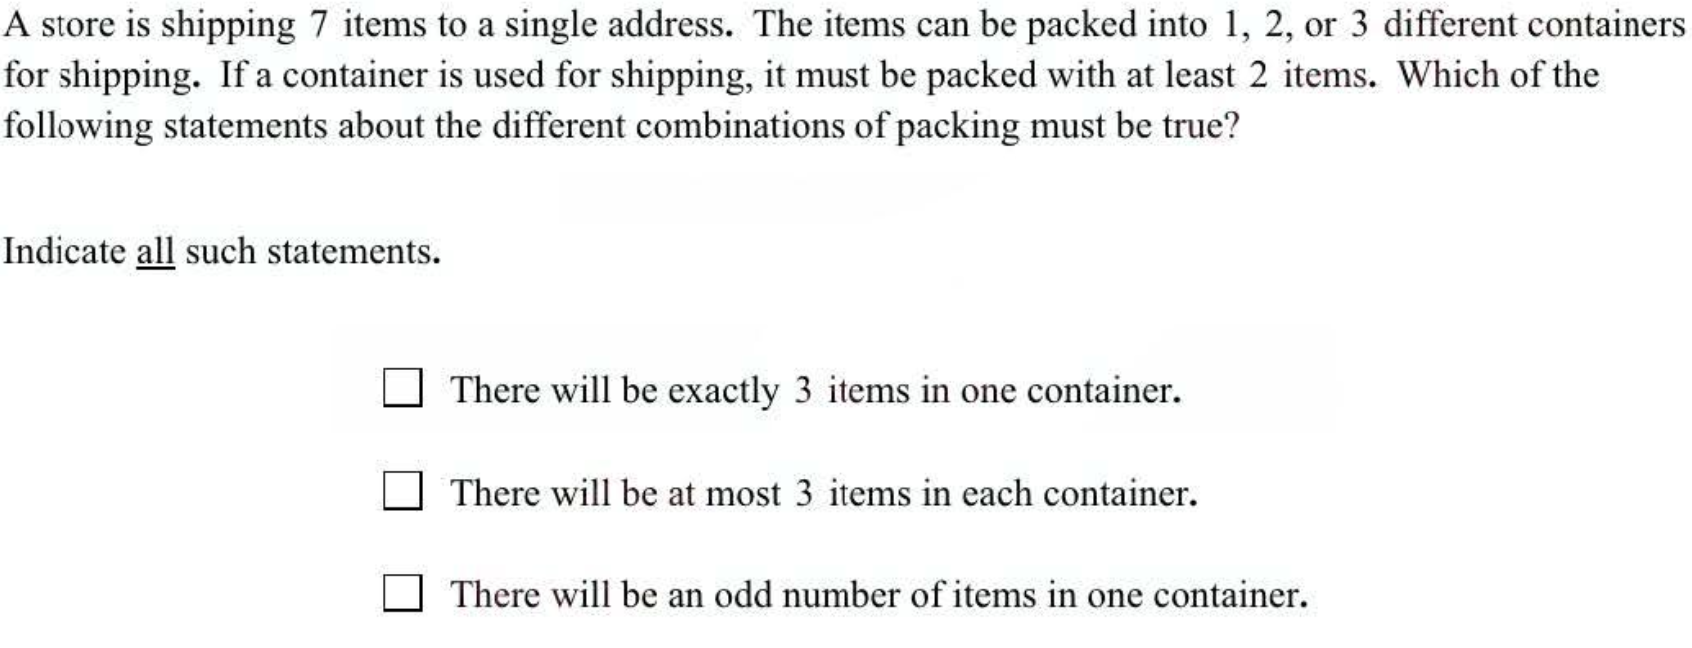
\includegraphics[width=\linewidth]{Combinations_Example_Question.png}
		\caption{9-Sec1-12}
	\end{figure}
	\pause
% $$ \\
\pause
\bigskip
Answer \textbf{B } 
\end{frame}

%------------------------------------------------
\section{Probability}

%------------------------------------------------

\subsection{Sets}

%------------------------------------------------

\subsection{Events}

%------------------------------------------------

\subsection{Mutually Inclusive Events}

%------------------------------------------------

\subsection{Independent Events}

%------------------------------------------------

\section{Descriptive Data Analysis (Exploratory Data Analysis)}

%------------------------------------------------
\begin{frame}
	\frametitle{To Begin With} % Slide title, remove this command for no title

	\begin{block}{QR Mathematical Convention 5}
		When graphical data presentations, such as bar graphs and line graphs,
are shown with scales, you should read, estimate, or compare quantities
by sight or by measurement, according to the corresponding scales.
	\end{block}

		\begin{block}{QR Mathematical Convention 4}
		Scales, grid lines, dots, bars, shadings, solid and dashed lines, legends,
etc., are used on graphs to indicate the data. Sometimes scales that do not
begin at 0 are used, and sometimes broken scales are used..
	\end{block}
	\begin{alertblock}{看图要点}
		\begin{itemize}
			\item Carefully understand title, the labels for x-axis and y-axis, and legends.看标题,XY轴,图例找到数据的含义
			\item Carefully examine the scales and unit.看单位
			\item Carefully examine the the starting point.看起点
		\end{itemize}
	\end{alertblock}
\end{frame}

%------------------------------------------------

\begin{frame}
	\frametitle{How to read a graph} % Slide title, remove this command for no title
	\framesubtitle{读图要点}
	\begin{figure}
		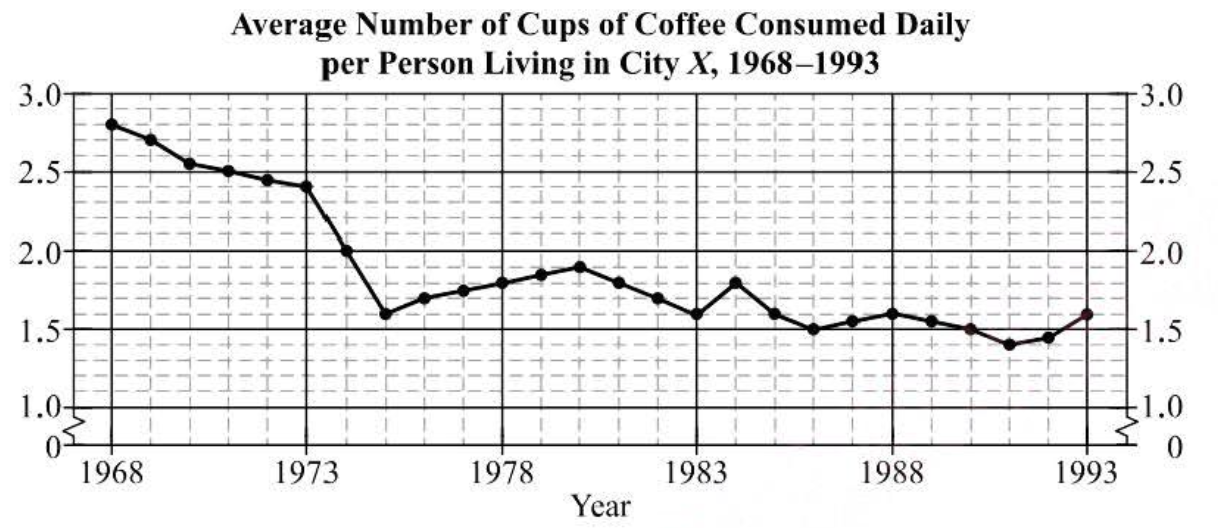
\includegraphics[width=0.8\linewidth]{Graph.png}
		\caption{The graph shows The trends of The average number of cups of coffee consumed daily
per person living in city X by year. Y suggest number of cups. X suggest the year. Y use a broken scales.}
	\end{figure}
\end{frame}

%------------------------------------------------


\subsection{Data Type}

%------------------------------------------------

%data distribution
\subsection{Methods for Presenting Data}

%------------------------------------------------

\subsection{Measures of Central Tendency}

%------------------------------------------------

\subsection{Measures of Position}

%------------------------------------------------

\subsection{Measures of Dispersion}

%------------------------------------------------


\section{Random Variables and Probability Distribution}

%------------------------------------------------

\subsection{Random Variables}

%------------------------------------------------

\subsection{Probability Distribution}

%------------------------------------------------

\subsection{Normal Distribution}

%------------------------------------------------



%------------------------------------------------
% 	\begin{columns}[t] 
% 		\begin{column}{0.5\textwidth} % Left column width
% 		\end{column}
% 		\begin{column}{0.5\textwidth} % Right column width
% 		\end{column}
% 	\end{columns}


% 	\begin{figure}
% 		
\includegraphics[width=0.8\linewidth]{creodocs_logo.pdf}
% 		\caption{Creodocs logo.}
% 	\end{figure}


% \begin{frame}
% 	\frametitle{A Real QR Problem!}
% 	\framesubtitle{}
% 	\begin{figure}
% 		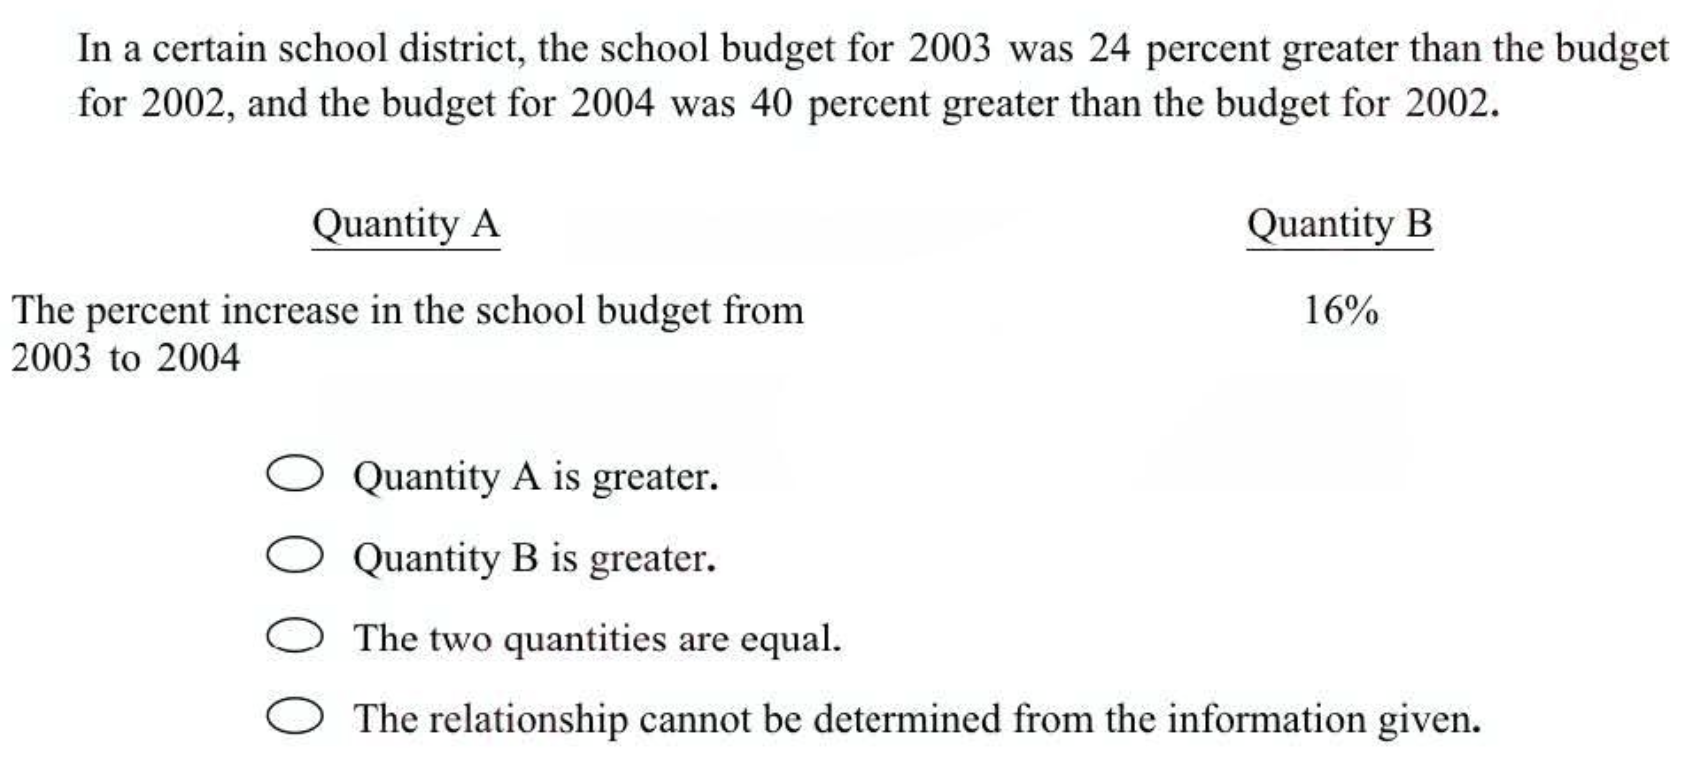
\includegraphics[width=\linewidth]{Percent_Increase_Example_Question1.png}
% 		\caption{-Sec-}
% 	\end{figure}
% 	\pause
% $$ \\
% \pause
% \bigskip
% Answer \textbf{B } 
% \end{frame}

% %------------------------------------------------


%------------------------------------------------

% \begin{frame}
% 	\frametitle{Have a try!}
% 	\framesubtitle{}


% \bigskip
% \pause

% \bigskip
% Answer \textbf{- 2.48\%}
% \end{frame}

% %------------------------------------------------
%------------------------------------------------
% \section{Text Examples} % Sections are added in order to organize your presentation into discrete blocks, all sections and subsections are automatically output to the table of contents as an overview of the talk but NOT output in the presentation as separate slides

% %------------------------------------------------

% \subsection{Paragraphs and Lists}

% \begin{frame}
% 	\frametitle{Paragraphs of Text}
	
% 	Sed iaculis \alert{dapibus gravida}. Morbi sed tortor erat, nec interdum arcu. Sed id lorem lectus. Quisque viverra augue id sem ornare non aliquam nibh tristique. Aenean in ligula nisl. Nulla sed tellus ipsum. Donec vestibulum ligula non lorem vulputate fermentum accumsan neque mollis.
	
% 	\bigskip % Vertical whitespace
	
% 	% Quote example
% 	\begin{quote}
% 		Sed diam enim, sagittis nec condimentum sit amet, ullamcorper sit amet libero. Aliquam vel dui orci, a porta odio.\\
% 		--- Someone, somewhere\ldots
% 	\end{quote}
	
% 	\bigskip % Vertical whitespace
	
% 	Nullam id suscipit ipsum. Aenean lobortis commodo sem, ut commodo leo gravida vitae. Pellentesque vehicula ante iaculis arcu pretium rutrum eget sit amet purus. Integer ornare nulla quis neque ultrices lobortis.
% \end{frame}

% %------------------------------------------------

% \begin{frame}
% 	\frametitle{Lists}
% 	\framesubtitle{Bullet Points and Numbered Lists} % Optional subtitle
	
% 	\begin{itemize}
% 		\item Lorem ipsum dolor sit amet, consectetur adipiscing elit
% 		\item Aliquam blandit faucibus nisi, sit amet dapibus enim tempus
% 		\begin{itemize}
% 			\item Lorem ipsum dolor sit amet, consectetur adipiscing elit
% 			\item Nam cursus est eget velit posuere pellentesque
% 		\end{itemize}
% 		\item Nulla commodo, erat quis gravida posuere, elit lacus lobortis est, quis porttitor odio mauris at libero
% 	\end{itemize}
	
% 	\bigskip % Vertical whitespace
	
% 	\begin{enumerate}
% 		\item Nam cursus est eget velit posuere pellentesque
% 		\item Vestibulum faucibus velit a augue condimentum quis convallis nulla gravida 
% 	\end{enumerate}
% \end{frame}

% %------------------------------------------------

% \subsection{Blocks}

% \begin{frame}
% 	\frametitle{Blocks of Highlighted Text}
	
% 	\begin{block}{Block Title}
% 		Lorem ipsum dolor sit amet, consectetur adipiscing elit. Integer lectus nisl, ultricies in feugiat rutrum, porttitor sit amet augue.
% 	\end{block}
	
% 	\begin{exampleblock}{Example Block Title}
% 		Aliquam ut tortor mauris. Sed volutpat ante purus, quis accumsan.
% 	\end{exampleblock}
	
% 	\begin{alertblock}{Alert Block Title}
% 		Pellentesque sed tellus purus. Class aptent taciti sociosqu ad litora torquent per conubia nostra, per inceptos himenaeos.
% 	\end{alertblock}
	
% 	\begin{block}{} % Block without title
% 		Suspendisse tincidunt sagittis gravida. Curabitur condimentum, enim sed venenatis rutrum, ipsum neque consectetur orci.
% 	\end{block}
% \end{frame}

% %------------------------------------------------

% \subsection{Columns}

% \begin{frame}
% 	\frametitle{Multiple Columns}
% 	\framesubtitle{Subtitle} % Optional subtitle
	
% 	\begin{columns}[t] 
% 		\begin{column}{0.5\textwidth} % Left column width
% 		\end{column}
% 		\begin{column}{0.5\textwidth} % Right column width
% 	\end{columns}





% \end{frame}

% %------------------------------------------------

% \section{Table and Figure Examples}

% \subsection{Table}

% \begin{frame}
% 	\frametitle{Table}
% 	\framesubtitle{Subtitle} % Optional subtitle
	
% 	\begin{table}
% 		\begin{tabular}{l l l}
% 			\toprule
% 			\textbf{Treatments} & \textbf{Response 1} & \textbf{Response 2}\\
% 			\midrule
% 			Treatment 1 & 0.0003262 & 0.562 \\
% 			Treatment 2 & 0.0015681 & 0.910 \\
% 			Treatment 3 & 0.0009271 & 0.296 \\
% 			\bottomrule
% 		\end{tabular}
% 		\caption{Table caption}
% 	\end{table}
% \end{frame}

% %------------------------------------------------

% \subsection{Figure}

% \begin{frame}
% 	\frametitle{Figure}
	
% 	\begin{figure}
% 		
\includegraphics[width=0.8\linewidth]{creodocs_logo.pdf}
% 		\caption{Creodocs logo.}
% 	\end{figure}





% \end{frame}

% %------------------------------------------------

% \section{Mathematics}

% \begin{frame}
% 	\frametitle{Definitions \& Examples}
	
% 	\begin{definition}
% 		A \alert{prime number} is a number that has exactly two divisors.
% 	\end{definition}
	
% 	\smallskip % Vertical whitespace
	
% 	\begin{example}
% 		\begin{itemize}
% 			\item 2 is prime (two divisors: 1 and 2).
% 			\item 3 is prime (two divisors: 1 and 3).
% 			\item 4 is not prime (\alert{three} divisors: 1, 2, and 4).
% 		\end{itemize}
% 	\end{example}
	
% 	\smallskip % Vertical whitespace
	
% 	You can also use the \texttt{theorem}, \texttt{lemma}, \texttt{proof} and \texttt{corollary} environments.
% \end{frame}

% %------------------------------------------------

% \begin{frame}
% 	\frametitle{Theorem, Corollary \& Proof}
	
% 	\begin{theorem}[Mass--energy equivalence]
% 		$E = mc^2$
% 	\end{theorem}
	
% 	\begin{corollary}
% 		$x + y = y + x$
% 	\end{corollary}
	
% 	\begin{proof}
% 		$\omega + \phi = \epsilon$
% 	\end{proof}
% \end{frame}

% %------------------------------------------------

% \begin{frame}
% 	\frametitle{Equation}

% 	\begin{equation}
% 		\cos^3 \theta =\frac{1}{4}\cos\theta+\frac{3}{4}\cos 3\theta
% 	\end{equation}
% \end{frame}

% %------------------------------------------------

% \begin{frame}[fragile] % Need to use the fragile option when verbatim is used in the slide
% 	\frametitle{Verbatim}
	
% 	\begin{example}[Theorem Slide Code]
% 		\begin{verbatim}
% 			\begin{frame}
% 				\frametitle{Theorem}
% 				\begin{theorem}[Mass--energy equivalence]
% 					$E = mc^2$
% 				\end{theorem}
% 		\end{frame}\end{verbatim} % Must be on the same line
% 	\end{example}
% \end{frame}

% %------------------------------------------------

% \begin{frame}
% 	Slide without title.
% \end{frame}

% %------------------------------------------------

% \section{Referencing}

% \begin{frame}
% 	\frametitle{Citing References}
	
% 	An example of the \texttt{\textbackslash cite} command to cite within the presentation:
	
% 	\bigskip % Vertical whitespace
	
% 	This statement requires citation \cite{p1,p2}.
% \end{frame}

% %------------------------------------------------

% \begin{frame} % Use [allowframebreaks] to allow automatic splitting across slides if the content is too long
% 	\frametitle{References}
	
% 	\begin{thebibliography}{99} % Beamer does not support BibTeX so references must be inserted manually as below, you may need to use multiple columns and/or reduce the font size further if you have many references
% 		\footnotesize % Reduce the font size in the bibliography
		
% 		\bibitem[Smith, 2022]{p1}
% 			John Smith (2022)
% 			\newblock Publication title
% 			\newblock \emph{Journal Name} 12(3), 45 -- 678.
			
% 		\bibitem[Kennedy, 2023]{p2}
% 			Annabelle Kennedy (2023)
% 			\newblock Publication title
% 			\newblock \emph{Journal Name} 12(3), 45 -- 678.
% 	\end{thebibliography}
% \end{frame}

% %----------------------------------------------------------------------------------------
% %	ACKNOWLEDGMENTS SLIDE
% %----------------------------------------------------------------------------------------

% \begin{frame}
% 	\frametitle{Acknowledgements}
	
% 	\begin{columns}[t] % The "c" option specifies centered vertical alignment while the "t" option is used for top vertical alignment
% 		\begin{column}{0.45\textwidth} % Left column width
% 			\textbf{Smith Lab}
% 			\begin{itemize}
% 				\item Alice Smith
% 				\item Devon Brown
% 			\end{itemize}
% 			\textbf{Cook Lab}
% 			\begin{itemize}
% 				\item Margaret
% 				\item Jennifer
% 				\item Yuan
% 			\end{itemize}
% 		\end{column}		
% 		\begin{column}{0.5\textwidth} % Right column width
% 			\textbf{Funding}
% 			\begin{itemize}
% 				\item British Royal Navy
% 				\item Norwegian Government
% 			\end{itemize}
% 		\end{column}
% 	\end{columns}
% \end{frame}

%----------------------------------------------------------------------------------------
%	CLOSING SLIDE
%----------------------------------------------------------------------------------------

\begin{frame}[plain] % The optional argument 'plain' hides the headline and footline
	\begin{center}
		{\Huge 1 Min Break}
		\bigskip\bigskip % Vertical whitespace
		
		{\LARGE Questions? Comments?}
	\end{center}
\end{frame}

%----------------------------------------------------------------------------------------

\end{document} 